\documentclass[12pt]{standalone}
\usepackage[utf8]{inputenc}
\usepackage[T1]{fontenc}
\usepackage{times}
\usepackage{amsmath,amssymb}
\usepackage[dvipsnames,svgnames]{xcolor}
\usepackage{tikz}
\usetikzlibrary{calc, arrows.meta}
\definecolor{winblue}{HTML}{0D366B}
\definecolor{inksec}{HTML}{52514E}
% Adaptado de Goldsmith (2004/2005), Fig. 5.18, p. 149 (4QAM e 16QAM): as duas constelacoes
% em paineis separados, na mesma escala e com a mesma energia media por simbolo
% (QPSK: +-a; 16-QAM: +-d, +-3d, com 10 d^2 = 2 a^2).
% Bits de cada ponto: mapeamento da TS 38.211 v18.6.0, Secs. 5.1.3 (QPSK, b0 b1) e 5.1.4
% (16QAM, b0 b1 b2 b3): I = (1-2b0)(2-(1-2b2)), Q = (1-2b1)(2-(1-2b3)).
\begin{document}
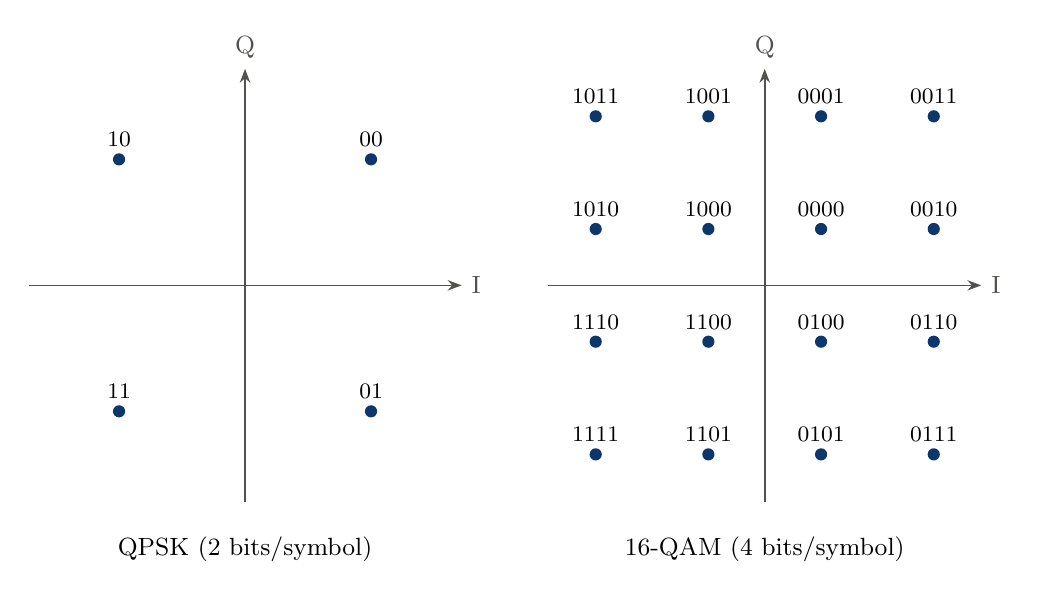
\begin{tikzpicture}[font=\fontsize{9}{10.8}\selectfont, >={Stealth[length=5pt]}]
\def\a{1.6}
\pgfmathsetmacro{\d}{\a/sqrt(5)}
\def\L{2.75}
% painel QPSK
\begin{scope}
  \draw[->, inksec, line width=0.6pt] (-\L,0) -- (\L,0) node[right] {I};
  \draw[->, inksec, line width=0.6pt] (0,-\L) -- (0,\L) node[above] {Q};
  \foreach \x/\y/\b in {1/1/00, 1/-1/01, -1/1/10, -1/-1/11} {
    \fill[winblue] (\x*\a,\y*\a) circle (2.2pt);
    \node[above=1pt, font=\fontsize{8}{9}\selectfont] at (\x*\a,\y*\a) {\b};
  }
  \node at (0,-\L-0.6) {QPSK (2 bits/symbol)};
\end{scope}
% painel 16-QAM
\begin{scope}[xshift=6.6cm]
  \draw[->, inksec, line width=0.6pt] (-\L,0) -- (\L,0) node[right] {I};
  \draw[->, inksec, line width=0.6pt] (0,-\L) -- (0,\L) node[above] {Q};
  \foreach \x/\y/\b in {1/1/0000, 1/3/0001, 3/1/0010, 3/3/0011, 1/-1/0100, 1/-3/0101, 3/-1/0110, 3/-3/0111, -1/1/1000, -1/3/1001, -3/1/1010, -3/3/1011, -1/-1/1100, -1/-3/1101, -3/-1/1110, -3/-3/1111} {
    \fill[winblue] (\x*\d,\y*\d) circle (2.2pt);
    \node[above=1pt, font=\fontsize{8}{9}\selectfont] at (\x*\d,\y*\d) {\b};
  }
  \node at (0,-\L-0.6) {16-QAM (4 bits/symbol)};
\end{scope}
\end{tikzpicture}
\end{document}
